\documentclass[%
 aip,
 jcp,
 amsmath,amssymb,
 preprint,%
%reprint,%
]{revtex4-1}


\usepackage{graphicx}
\usepackage{dcolumn}
\usepackage{bm}
\usepackage[utf8]{inputenc}
\usepackage[T1]{fontenc}

%\usepackage{hyperref}
\usepackage[hidelinks]{hyperref}
\graphicspath{{generated/figures/}}
\usepackage{float}
\renewcommand{\topfraction}{0.95}
\renewcommand{\bottomfraction}{0.95}
\renewcommand{\textfraction}{0.05}
\renewcommand{\floatpagefraction}{0.85}
\setcounter{topnumber}{4}
\setcounter{bottomnumber}{4}
\setcounter{totalnumber}{8}
\usepackage[usenames,dvipsnames]{xcolor}
\usepackage[normalem]{ulem}
\definecolor{RED}{named}{red}
\usepackage{tikz}
\usepackage{mathtools}
\usepackage{booktabs}
\usepackage{siunitx}
\usepackage{multirow}
\usepackage{subcaption}
\usepackage{verbatim}
\usepackage{stmaryrd}
\usepackage{xr}
\externaldocument[MAIN-]{main}

\begin{document}

\title{Supplementary Material for: Hierarchical Bayesian calibration of mesoscopic models for ultrasound contrast agents from force spectroscopy data}

\author{Brieuc Benvegnen}
\thanks{These authors contributed equally to this work.}
\affiliation{Universitat de Barcelona Institute of Complex Systems (UBICS),
C/ Martí i Franqués 1, 08028 Barcelona, Spain}

\author{Nikolaos Ntarakas}
\thanks{These authors contributed equally to this work.}
\affiliation{Theory Department, National Institute of Chemistry,
Hajdrihova 19, 1001 Ljubljana, Slovenia}
\affiliation{Department of Physics, Faculty of Mathematics and Physics,
University of Ljubljana, Jadranska 19, 1000 Ljubljana, Slovenia}

\author{Tilen Potisk}
\affiliation{Theory Department, National Institute of Chemistry,
Hajdrihova 19, 1001 Ljubljana, Slovenia}
\affiliation{Department of Physics, Faculty of Mathematics and Physics,
University of Ljubljana, Jadranska 19, 1000 Ljubljana, Slovenia}

\author{Ignacio Pagonabarraga}
\affiliation{Universitat de Barcelona Institute of Complex Systems (UBICS),
C/ Martí i Franqués 1, 08028 Barcelona, Spain}

\author{Matej Praprotnik}
\email[Author to whom correspondence should be addressed: ]{praprot@cmm.ki.si}
\affiliation{Universitat de Barcelona Institute of Complex Systems (UBICS),
C/ Martí i Franqués 1, 08028 Barcelona, Spain}
\affiliation{Theory Department, National Institute of Chemistry,
Hajdrihova 19, 1001 Ljubljana, Slovenia}
\affiliation{Department of Physics, Faculty of Mathematics and Physics,
University of Ljubljana, Jadranska 19, 1000 Ljubljana, Slovenia}


\setcounter{section}{0}
\setcounter{equation}{0}
\setcounter{table}{0}
\setcounter{figure}{0}

\renewcommand{\thesection}{S\arabic{section}}
\renewcommand{\theequation}{S\arabic{equation}}
\renewcommand{\thetable}{S\arabic{table}}
\renewcommand{\thefigure}{S\arabic{figure}}

\maketitle

\section{\texorpdfstring{\textsc{dpd}}{DPD} Model Implementation Details}
\label{app:dpd_details}

Each microbubble shell is represented as a triangulated surface whose vertex positions, connectivity, and reference geometric quantities are generated before the \textsc{dpd} run starts \cite{ntarakas2025dissipative}. Relevant setup scripts build a diameter-dependent shell geometry, write the corresponding parameter files, and prepare the simulation environment used later by the inference and propagation workflows. In that sense, the shell geometry used in the paper is not an abstract analytical construction separate from the codebase: it is the same geometry that is generated and subsequently used by the simulations. Microbubble meshes were loaded from pre-generated triangulations and immersed in a solvent domain containing explicit water and gas particles. This choice of experimental conditions aligns with force spectroscopy studies, which are conducted in liquid environments to preserve structural integrity and avoid mechanical artifacts associated with drying \cite{buchner2012}. Compression and indentation use the same shell force field but different loading prescriptions. In compression, the shell is loaded through a plate-based contact geometry and the observable of interest is the reaction force as a function of imposed displacement. In indentation, the shell is loaded by prescribed pole forces and the observable is the resulting displacement as a function of applied force. This difference is carried consistently through the entire workflow: the compression \textsc{dnn} surrogates are trained in the forward direction `force(displacement, parameters)`, whereas the indentation \textsc{dnn} surrogates are trained in the inverse direction `displacement(force, parameters)`. In both compression and indentation setups, simulations consisted of an equilibration phase followed by a sampling phase. Forces were averaged over the final portion of each run to reduce thermal noise. Typical simulations used time steps of $\Delta t = 0.0001$, total durations of $10^5 - 10^6$ steps, and required approximately 30--60 minutes per run on a single \textsc{nvidia} A40 \textsc{gpu}. \textsc{map} responses were evaluated at 15 displacement points per diameter. Each point used $n_\mathrm{steps} = 20{,}000$ integration steps after $n_\mathrm{eq} = 40{,}000$ equilibration steps, matching the conditions used during \textsc{dnn} surrogate training data generation.

\newpage
\section{Experimental force spectroscopy data}
\label{app:exp_details}

In this work, we are using experimental force spectroscopy data from published literature. In these experiments, \textsc{afm} was used to investigate the mechanical properties of individual SonoVue\textsuperscript{\textregistered} microbubbles via indentation with a tipped cantilever. The experiments followed protocols described in detail by Morris~\cite{morris2014mechanical}. Individual \textsc{emb}s were imaged and targeted using an inverted optical microscope. A sharp-tipped cantilever was employed, with a nominal tip radius of 20 nm and calibrated spring constants obtained using inverse optical lever sensitivity measurements followed by the thermal noise method. The experiments were performed in aqueous conditions, using an Asylum Research MFP-1D \textsc{afm} system with Bruker MLCT AUNM tipped cantilevers (Bruker \textsc{afm} probes, Camarillo, CA) with nominal spring constants $k_c = 0.005$--$0.025$~N/m. The cantilever approach and retraction were performed at a constant speed of $3~\mu$m/s. To ensure precise measurement of local shell deformation, force spectroscopy was performed by advancing the \textsc{afm} tip toward the apex of each microbubble at a controlled rate, generating force--displacement ($F$--$\Delta$) curves. Both approach and retract curves were collected, but only the approach segment was used for fitting, as it corresponds to the compressive phase. The deformation was limited to ensure an elastic response and avoid structural damage. Since the applied force in \textsc{afm} is determined from cantilever deflection using Hooke's law, the cantilever spring constant serves only as a measurement parameter and does not influence the intrinsic membrane response. Consistent with this, experimental studies report only a weak dependence of the inferred mechanical properties on cantilever stiffness or probe geometry \cite{morris2014mechanical}. Accordingly, our simulations, which model the intrinsic force--deformation behavior of the membrane, are expected to be insensitive to the specific cantilever stiffness used in the experiments.

Tipless cantilevers were used to apply parallel-plate compression to individual Definity\textsuperscript{\textregistered} microbubbles, as described by Buchner-Santos et al.~\cite{buchner2012}. The \textsc{emb}s were immobilized at the base of poly-L-lysine coated Petri dishes via a passive float-and-adhere protocol to maintain their structural integrity. All force measurements were performed in deionized water using an Asylum Research MFP-1D \textsc{afm} system mounted on an inverted optical microscope (Nikon TE2000U). Tipless rectangular cantilevers (spring constants $k_c = 0.07$--$0.25$~N/m) with aluminum backside coating were used to compress \textsc{emb}s at a constant speed of approximately $6~\mu$m/s. The cantilever deflection and piezoelectric displacement were recorded, allowing calculation of the applied force and \textsc{emb} deformation. 

The two commercial agents also differ in shell composition. Definity contains a lipid shell based on DPPC, DPPA, and PEGylated DPPE, whereas SonoVue contains DSPC, DPPG, palmitic acid, and PEG/macrogol-containing components. Here, we reanalyze published experimental force--displacement curves after conversion to \textsc{dpd} units and preprocessing specific to each \textsc{emb} type. Each posterior is conditioned on one representative published curve per diameter. Because the workflow repository stores only the representative curve actually used for inference, rather than the full original experimental cohorts, Table~\ref{tab:data_summary} reports the number of curves used by the inference workflow and the retained point counts, not the total number of bubbles measured in the source studies.

\begin{figure}[H]
\centering
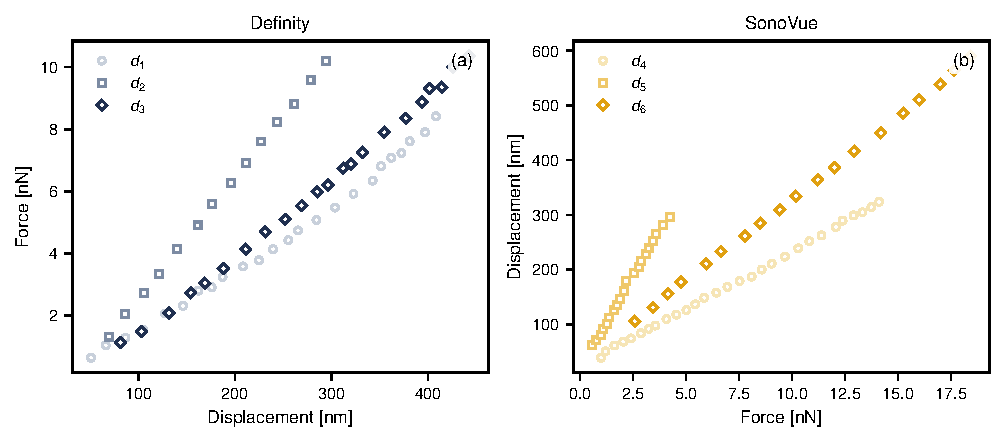
\includegraphics[width=\textwidth]{Figure_S1.pdf}
\caption{Experimental reference curves used throughout the calibration workflow, shown in real units. Panel (a) shows compression data (ink) and panel (b) shows indentation data (gold). Each curve corresponds to a reprocessed published loading branch (Refs.~\cite{buchner2012,morris2014mechanical}) and serves as the diameter-specific target for \textsc{dnn} surrogate evaluation, Bayesian inference, and posterior predictive propagation.}
\label{fig:reference_curves}
\noindent\textbf{Alt text:} Experimental reference curves used as calibration targets. Definity compression and SonoVue indentation data are shown for the six diameter-specific datasets.
\end{figure}


\section{Experimental acoustic data}
\label{app:resonance_data}

The resonance-frequency data summarized in Table~\ref{tab:resonance_data_summary} were extracted from two experimental studies that employed optical observations of individual microbubbles. For SonoVue, van der Meer \textit{et al.}~\cite{vandermeer2004sonovue} determined the resonance frequency by sweeping the excitation frequency between 1.5 and 5.0~MHz and identifying the frequency at which the normalized radial excursion, $R_{\max}/R_0$, reached its maximum. They used 160~kHz increments while keeping the acoustic pressure constant at 130~kPa. At each frequency, the bubble was insonified with an 8-cycle pulse. For Definity, Goertz \textit{et al.}~\cite{goertz2006pulse} used 10~MHz excitation pulses and determined the resonance frequency either from the bubble's free oscillation following a single pulse or from the pulse repetition frequency that produced the largest radial oscillation during repeated excitation.

\begin{table}[!htbp]
\caption{\label{tab:resonance_data_summary}
Published acoustic-frequency observations used in the acoustically constrained hierarchy.}
\noindent\textbf{Alt text:} Table of bubble diameters and fundamental acoustic frequencies used as additional calibration data for Definity and SonoVue.
\par\vspace{0.75\baselineskip}
\begin{center}
\scriptsize
\begin{tabular}{llll}
\hline
Agent & Source label & Diameter [$\mu$m] & Frequency [MHz] \\
\hline
SonoVue & van der Meer et al.\ \cite{vandermeer2004sonovue}, Fig. 2 & 2.6 & 3.10 \\
SonoVue & van der Meer et al.\ \cite{vandermeer2004sonovue}, Fig. 2 & 3.2 & 2.10 \\
SonoVue & van der Meer et al.\ \cite{vandermeer2004sonovue}, Fig. 2 & 4.0 & 1.60 \\
Definity & Goertz et al.\ \cite{goertz2006pulse}, Fig. 3 & 4.68 & 1.69 \\
Definity & Goertz et al.\ \cite{goertz2006pulse}, Fig. 3 & 5.18 & 1.70 \\
Definity & Goertz et al.\ \cite{goertz2006pulse}, Fig. 3 & 5.59 & 1.49 \\
Definity & Goertz et al.\ \cite{goertz2006pulse}, Fig. 3 & 6.00 & 1.49 \\
Definity & Goertz et al.\ \cite{goertz2006pulse}, Fig. 3 & 6.18 & 1.06 \\
Definity & Goertz et al.\ \cite{goertz2006pulse}, Fig. 3 & 7.08 & 1.06 \\
Definity & Goertz et al.\ \cite{goertz2006pulse}, Fig. 3 & 7.20 & 1.50 \\
Definity & Goertz et al.\ \cite{goertz2006pulse}, Fig. 3 & 7.29 & 0.90 \\
Definity & Goertz et al.\ \cite{goertz2006pulse}, Fig. 3 & 7.86 & 0.91 \\
Definity & Goertz et al.\ \cite{goertz2006pulse}, Fig. 3 & 8.67 & 0.80 \\
Definity & Goertz et al.\ \cite{goertz2006pulse}, Fig. 3 & 8.87 & 0.90 \\
Definity & Goertz et al.\ \cite{goertz2006pulse}, Fig. 3 & 10.00 & 0.80 \\
Definity & Goertz et al.\ \cite{goertz2006pulse}, Fig. 3 & 10.09 & 0.58 \\
Definity & Goertz et al.\ \cite{goertz2006pulse}, Fig. 3 & 11.20 & 0.58 \\
\hline
\end{tabular}
\end{center}
\end{table}


\section{Forward-model details for hierarchical inference}
\label{app:hierarchical_derivation}

This section specifies the experiment-dependent surrogate maps used in the Bayesian calibration workflow. The general likelihood, prior structure, and staged hierarchical inference procedure are given in the Methods section. For Definity \textsc{emb}s, the mechanical surrogates $\mathcal{S}_{d_1}, \mathcal{S}_{d_2}$ and $\mathcal{S}_{d_3}$ approximate the compression forward map
  \begin{equation}
    \bigl(k_a, k_b, b_1, b_2, a_3, a_4, d\bigr) \;\mapsto\; F,
  \end{equation}
  that is, the compressive force $F$ at displacement $d$ for a given set of material parameters. For SonoVue \textsc{emb}s, the mechanical surrogates $\mathcal{S}_{d_4},
  \mathcal{S}_{d_5}$ and $\mathcal{S}_{d_6}$ approximate the indentation forward map
  \begin{equation}
    \bigl(k_a, k_b, b_1, b_2, a_3, a_4, F\bigr) \;\mapsto\; d,
  \end{equation}
  that is, the indentation displacement $d$ at applied force $F$ for a given set of material parameters.
  
Before inference, each published reference curve is reduced to the subset that actually enters the likelihood (see Fig.~\ref{fig:reference_curves}), and Table~\ref{tab:data_summary} explicitly reports the corresponding retained point counts. In both cases of \textsc{emb}s, the retained points correspond to the linear loading regions defined in the respective reference experimental papers. The published curves are read or converted into \textsc{dpd} units and written as diameter-specific files used by the workflow, with no interpolation or additional manual alignment shift introduced afterward.

The displacement offset $d_0$ is added as an additional degree of freedom of the model, shifting all displacements so that the model encompasses the experimental uncertainty regarding the establishment of the bubble-cantilever contact. It is taken into account in an experiment-dependent way. For compression, we shift the experimental displacement before mechanical surrogate evaluation,
\begin{equation}
\tilde{x}_{ij} = \max(0, x_{ij} - d_{0,i}), \qquad
\hat{y}_{ij} = \mathcal{S}_{d_i}(\Theta_i;\tilde{x}_{ij}),
\end{equation}
where $(\mathcal{S}_{d_i})_{i=1,2,3}$ maps $(k_a,k_b,b_1,b_2,a_3,a_4,\tilde{x}) \mapsto F$.
For indentation, the mechanical surrogate predicts displacement as a function of force and parameters, and we apply the offset as an additive shift on the predicted displacement,
\begin{equation}
\hat{y}_{ij} = \hat{d}_{ij} = \mathcal{S}_{d_i}(\Theta_i;x_{ij}) + d_{0,i},
\end{equation}
where $(\mathcal{S}_{d_i})_{i=4,5,6}$ maps $(k_a,k_b,b_1,b_2,a_3,a_4,F) \mapsto d$. This asymmetry reflects the native mechanical surrogate parameterizations used in the workflow: compression surrogates predict force at a prescribed displacement, whereas indentation surrogates predict displacement at a prescribed force. In both cases, non-negativity is enforced at evaluation time by clamping predictions to zero when necessary (no negative compressive force and no negative indentation depth).

At the hierarchical stage, each mechanical and acoustic dataset has its own latent parameter vector and observation-noise amplitude and contributes a separate marginal likelihood to the \textsc{emb}-specific hyperparameter posterior:
\begin{equation}
P(\psi \mid \{\mathcal{D}_i\},\{f_j\})
\propto
P(\psi)\prod_{i=1}^{3} P(\mathcal{D}_i \mid \psi)
\prod_j P(f_j \mid \psi),
\end{equation}
where the mechanical marginal is
\begin{equation}
P(\mathcal{D}_i \mid \psi)
=
\int
P(\mathcal{D}_i \mid \Theta_i,\sigma_i^{\mathrm{mech}})\,
P(\Theta_i \mid \psi)\,
P(\sigma_i^{\mathrm{mech}})\,
d\Theta_i\, d\sigma_i^{\mathrm{mech}}.
\end{equation}
For an acoustic observation at diameter $d_j$, the corresponding marginal is
\begin{equation}
P(f_j\mid\psi)
=
\int
P(f_j\mid \Theta_j,\sigma_j^{\mathrm{ac}})\,
P(\Theta_j\mid\psi)\,
P(\sigma_j^{\mathrm{ac}})\,
d\Theta_j\,d\sigma_j^{\mathrm{ac}}.
\end{equation}
Here, the acoustic surrogate gives $\hat f_j=\mathcal{A}_{d_j}(k_{a,j})$, and the relative Gaussian observation model is $P(f_j\mid\Theta_j,\sigma_j^{\mathrm{ac}})=\mathcal{N}\!\left(f_j\,\middle|\,\hat f_j,[\sigma_j^{\mathrm{ac}}\hat f_j]^2\right)$.

\section{Mechanical and acoustic surrogates}
\label{app:surrogate}

\subsection{DNN surrogates for force-displacement simulations}
Training data are generated by sampling the force field parameter space using Latin Hypercube Sampling \cite{joseph2020designing} and evaluating the corresponding \textsc{dpd} simulations at a prescribed set of loading points. Sampling is managed through the \textsc{korali} engine (distributed \textsc{mpi} execution) and produces diameter-specific datasets for training the \textsc{dnn} surrogates. Across the six diameter-specific surrogate datasets considered here, the training sets contain approximately $5\times10^3$ to $10^4$ simulated samples per diameter. For compression, each training sample consists of a parameter vector and a sequence of displacement points with the associated simulated forces, while for indentation, each training sample consists of a parameter vector and a sequence of forces with the associated recorded displacements. In both cases, the raw simulated curves are filtered before training to remove invalid or non-physical entries and enforce consistency in the force--displacement relationship: simulated curves exhibiting abrupt force drops indicative of bubble rupture events are removed using a monotonicity-based criterion prior to architecture selection. \\
Each \textsc{dnn} surrogate is a fully connected multilayer perceptron (\textsc{mlp}) with $\tanh$ activations and Xavier initialization \cite{glorot2010understanding} for the linear-layer weights. For each \textsc{emb} diameter, we perform an architecture sweep over a fixed set of widths and depths and select the best model based on validation performance. Specifically, we evaluate 12 candidate \textsc{mlp}s spanning widths $\{32,64,128,256\}$ and depths $\{2,3,4\}$, train all candidates, and retain the model with the lowest grouped-holdout median relative $L^2$ error. The selected grouped-holdout architectures are $(128,4)$, $(128,4)$, and $(128,3)$ for compression diameters 2.1, 2.9, and $3.0~\mu$m, and $(32,3)$, $(256,3)$, and $(128,4)$ for indentation diameters 3.2, 3.4, and $5.8~\mu$m, respectively. Fig.~\ref{fig:surrogate_group_holdout_examples} displays one representative held-out curve per diameter, chosen near the median grouped-holdout relative error. The points denote held-out \textsc{dpd} data excluded from training, and the lines denote the \textsc{dnn} surrogate predictions. Inputs and targets are standardized using the feature-wise mean and standard deviation computed from the training dataset, and the normalization parameters are stored alongside the trained PyTorch \cite{ansel2024pytorch} model in a pickle file. A 90/10 pointwise split is used to monitor training. Architecture selection uses the grouped-holdout score. The models are trained with the Adam optimizer \cite{kingma2014adam} and \textsc{mse} loss. Training includes a validation-based learning rate reduction mechanism: when the validation loss does not improve for a fixed patience window, the learning rate is reduced by a factor of $10$ and training continues. The procedure stops after a fixed number of reduction rounds or when the maximum number of epochs is reached. Unless otherwise stated, training is performed on \textsc{cpu}s. For reduced-model analyses in which $(b_1,b_2,a_3,a_4)$ are fixed to zero, we reuse the same trained \textsc{dnn} surrogates and evaluate them with these inputs set to zero, rather than retraining separate reduced surrogates.

\begin{figure}[H]
\centering
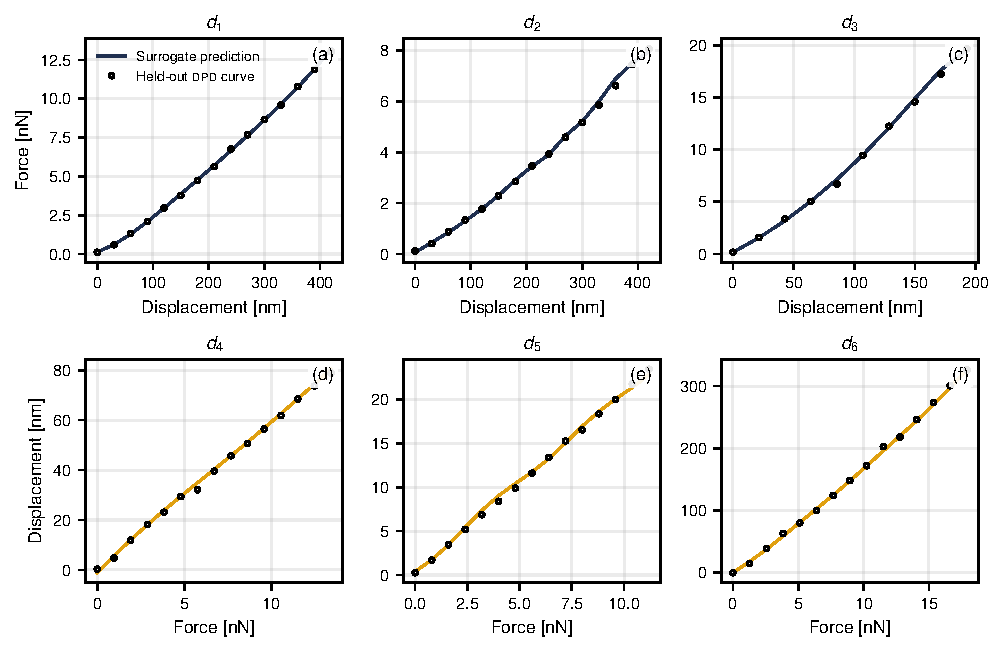
\includegraphics[width=\textwidth]{Figure_S3.pdf}
\caption{Grouped parameter-set holdout validation for all six \textsc{dnn} surrogates in real units. Each panel shows one representative held-out curve chosen near the median grouped-holdout relative $L^2$ error for that diameter. Points denote held-out \textsc{dpd} responses excluded from training, and lines denote the \textsc{dnn} surrogate predictions. Compression panels report reaction force as a function of displacement; indentation panels report displacement as a function of applied force. Panels (a–c) depict Definity (ink), and panels (d–f) depict SonoVue (gold).}
\label{fig:surrogate_group_holdout_examples}
\noindent\textbf{Alt text:} Grouped-holdout validation curves for all six \textsc{dnn} surrogates. Each panel compares a held-out DPD response with the corresponding DNN surrogate prediction for one bubble diameter.
\end{figure}

\subsection{DPD-fitted polynomial acoustic surrogates}
\label{app:resonance_forward_map}

For each simulated diameter $d_i$, the squared resonance frequency is represented as
\begin{equation}
\label{eq:si_acoustic_surrogate}
f_{\mathrm{res},d_i}^2(k_a)
=a_{0,d_i}+a_{1,d_i}k_a+a_{2,d_i}k_a^2.
\end{equation}
The surrogate $\mathcal{A}_{d_i}(k_a)$ then predicts the value of $f_{\mathrm{res}}$ given by this fitted relation.

\begin{figure}[!t]
\centering
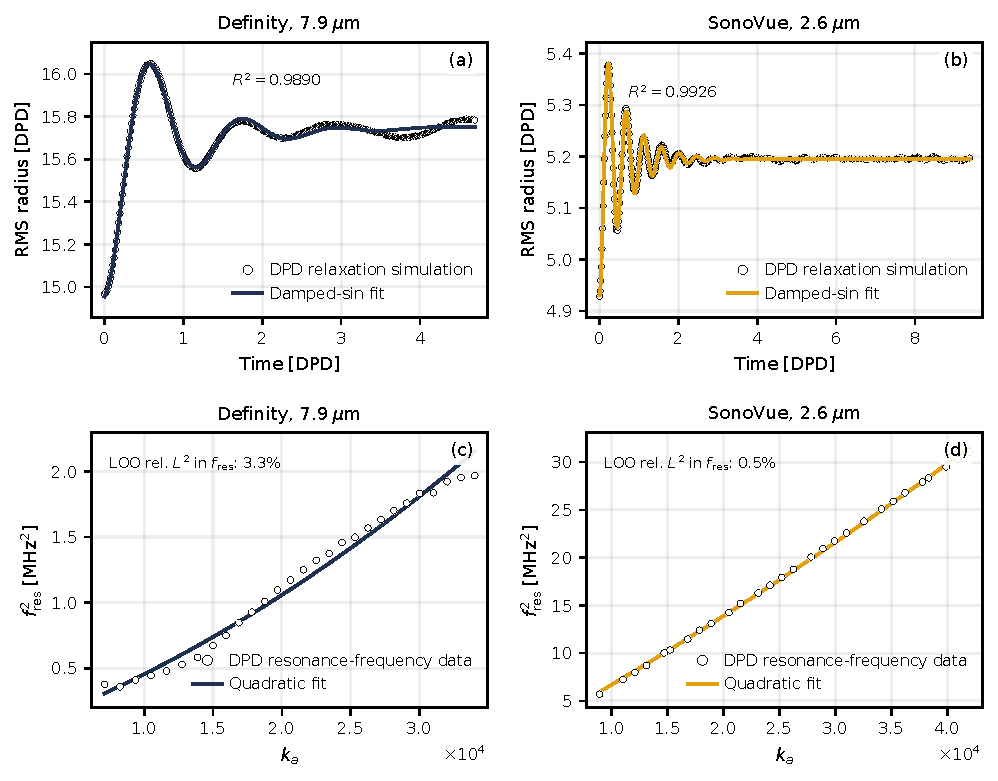
\includegraphics[width=\textwidth]{Figure_S2.pdf}
\captionsetup{justification=raggedright,singlelinecheck=false}
\caption{Representative \textsc{dpd} ringdowns and polynomial acoustic surrogates. Panels (a) and (b) show Definity at $7.9~\mu$m and SonoVue at $2.6~\mu$m, respectively. Open black circles denote sampled root-mean-square membrane radii, and the colored curves denote the damped-sine fits
$R(t)=R_0+ct+\exp(-\lambda t)[A\sin(\omega_d t)+B\cos(\omega_d t)]$. Panels (c) and (d) show the squared resonance frequencies extracted from the \textsc{dpd} ringdowns as functions of $k_a$ and the corresponding quadratic polynomial surrogates; the reported relative $L^2$ errors in $f_{\mathrm{res}}$ are from leave-one-out validation.}
\label{fig:si_ringdown_fit_examples}
\noindent\textbf{Alt text:} Representative Definity and SonoVue DPD radius-relaxation samples with damped-sine fits, followed by squared resonance frequencies against $k_a$ with quadratic polynomial surrogates and leave-one-out errors.
\end{figure}

The ringdown fits used to obtain $\omega_d$ and $\lambda$ are shown in Fig.~\ref{fig:si_ringdown_fit_examples}(a) and (b), while panels (c) and (d) show the corresponding frequency sweeps and polynomial surrogates. In the fit, $R_0$ is the equilibrium radius, $c$ is the linear drift, $A$ and $B$ are the oscillation amplitudes, $\lambda$ is the decay rate, and $\omega_d$ is the damped angular frequency. For these sweeps, $k_a$ was varied with the coupled shear modulus $\mu=k_a/3$, while the remaining simulation conditions were fixed, including $k_b=389.23$ for Definity and $k_b=7850.29$ for SonoVue. The membrane mass was multiplied by a factor of 160 to obtain stable ringdowns with enough oscillations for fitting. At this simulated mass scale, the damped, natural, and resonance frequencies are $f_d=\omega_d/(2\pi)$, $f_0=(\omega_d^2+\lambda^2)^{1/2}/(2\pi)$, and $f_{\mathrm{res}}=(\omega_d^2-\lambda^2)^{1/2}/(2\pi)$, respectively. The resulting $f_{\mathrm{res}}$ values were multiplied by $\sqrt{160}$ to recover the physical-mass frequencies used to fit the polynomial surrogates. Matched-coordinate mass sweeps numerically confirmed the expected inverse-square-root frequency scaling, $f\propto M^{-1/2}$, consistent with $f=\sqrt{K/M}$.

At each simulated diameter, each of the 28 retained \textsc{dpd} frequency values was omitted in turn, the polynomial was refitted to the other 27 frequencies, and the omitted value was predicted.

\section{\textsc{tmcmc}}
\label{app:tmcmc}
We perform Bayesian parameter inference using \textsc{tmcmc}~\citep{ching2007transitional}, a population-based algorithm that bridges the prior to the posterior through a sequence of intermediate densities,
\begin{equation}
\rho_j(\Theta_i) \propto p(\Theta_i)\, p(\mathcal{D}_i|\Theta_i)^{p_j}, \qquad 0 = p_0 < p_1 < \cdots < p_J = 1
\end{equation}
where $p(\Theta_i)$ denotes the prior, $p(\mathcal{D}_i|\Theta_i)$ the likelihood, and $\{p_j\}$ the annealing schedule. Thus, $p_0=0$ gives the prior and $p_J=1$ gives the posterior. Starting with samples drawn from the prior, \textsc{tmcmc} iteratively increases the annealing exponent to shift probability mass toward regions of high likelihood. At each stage, samples from $\rho_j$ are reweighted according to the incremental tempering step (effectively using weights proportional to $p(\mathcal{D}_i|\Theta_i)^{p_{j+1}-p_j}$), resampled to control weight degeneracy, and then ``rejuvenated'' with a Markov chain kernel targeting $\rho_{j+1}$. Repeating this procedure until $p_J=1$ yields an empirical approximation of the posterior distribution.

In our implementation, \textsc{tmcmc} is provided by the \textsc{korali} framework~\citep{martin2022korali} and executed in parallel using \textsc{mpi}. \textsc{korali} manages the annealing schedule, importance reweighting and resampling between stages, and distributed evaluation of the forward model across the population. The annealing increments are selected adaptively using a target coefficient of variation (CoV) for the incremental importance weights: a larger target CoV allows larger increases in $p_j$ (fewer tempering stages but more variable weights), while a smaller target CoV enforces smaller increments (more stages and a more gradual transition). Within each stage, the Markov chain proposal is based on the (weighted) population covariance, scaled by a user-defined covariance scaling factor. This parameter controls the typical proposal step size, balancing mixing (too small leads to slow exploration) against acceptance (too large leads to frequent rejections).

The \textsc{tmcmc} settings used in this work are a population size of 50{,}000, a CoV of 0.8 (single-level inference) and 0.6 (hyperparameter inference, hierarchical-specific posteriors), and a covariance scaling parameter of 0.04 (all inference phases).

\clearpage
\section{Sensitivity analysis}
\label{app:sensitivity}
First-order Sobol indices were computed using \textsc{SALib}
\cite{herman2017salib} via the Saltelli estimator with $N = 2,048$
samples drawn over the prior ranges listed in Table~\ref{tab:priors}, using the full \textsc{dnn} surrogate (with nonlinear terms
active). Indices were computed pointwise along the loading branch and
then averaged over the experimentally explored range, as described in
Section~III B in the main text.

\section{Parameters and validation tables}
\begin{table}[!htbp]
\caption{\label{tab:surrogate_validation}
\textsc{dnn} surrogate validation summary for all six diameters. We report only the grouped-holdout median relative $L^2$ error from the stricter parameter-set holdout audit, in which whole simulated curves are excluded from training.}
\noindent\textbf{Alt text:} DNN-surrogate validation summary for all six diameters. Median grouped-holdout relative L2 errors remain low for both compression and indentation DNN surrogates.
\par\vspace{0.75\baselineskip}
\begin{ruledtabular}
\begin{tabular}{lllcc}
Agent & Bubble & Diameter [$\mu$m] & Setup & Grouped-holdout median rel.\ $L^2$ [\%] \\
\hline
Definity & $d_1$ & 2.1 & Compression & 0.92 \\
Definity & $d_2$ & 2.9 & Compression & 2.09 \\
Definity & $d_3$ & 3.0 & Compression & 2.06 \\
\hline
SonoVue & $d_4$ & 3.2 & Indentation & 2.20 \\
SonoVue & $d_5$ & 3.4 & Indentation & 2.55 \\
SonoVue & $d_6$ & 5.8 & Indentation & 1.55 \\
\end{tabular}
\end{ruledtabular}
\end{table}

\begin{table}[!htbp]
\caption{\label{tab:data_summary}
Experimental datasets used for inference.
Each posterior is conditioned on one reprocessed published curve per diameter.
``Source points'' denotes the number of points parsed from the published/source
curve before \textsc{dpd}-unit conversion and trimming.
``Retained points'' denotes the number of points in the processed curve actually
used by the inference workflow.
Source references are cited in the table.}
\noindent\textbf{Alt text:} Summary of the experimental datasets used for inference. The table identifies the source, agent, diameter, number of reprocessed curves, and retained data points for each calibration target.
\par\vspace{0.75\baselineskip}
\begin{ruledtabular}
\scriptsize
\resizebox{\textwidth}{!}{%
\begin{tabular}{lllclcccl}
Agent &
Bubble &
Diameter [$\mu$m] &
Type &
\shortstack{Source\\reference} &
\shortstack{Curves\\used} &
\shortstack{Source\\points} &
\shortstack{Retained\\points} &
\shortstack{Input\\type} \\
\hline
Definity & $d_1$ & 2.1 & Compression & Buchner-Santos et al.~\cite{buchner2012} & 1 & 27 & 24 & Reprocessed \\
Definity & $d_2$ & 2.9 & Compression & Buchner-Santos et al.~\cite{buchner2012} & 1 & 17 & 14 & Reprocessed \\
Definity & $d_3$ & 3.0 & Compression & Buchner-Santos et al.~\cite{buchner2012} & 1 & 25 & 22 & Reprocessed \\
\hline
SonoVue & $d_4$ & 3.2 & Indentation & Morris~\cite{morris2014mechanical} & 1 & 32 & 29 & Reprocessed \\
SonoVue & $d_5$ & 3.4 & Indentation & Morris~\cite{morris2014mechanical} & 1 & 46 & 20 & Reprocessed \\
SonoVue & $d_6$ & 5.8 & Indentation & Morris~\cite{morris2014mechanical} & 1 & 22 & 19 & Reprocessed \\
\end{tabular}%
}
\end{ruledtabular}
\end{table}

\begin{table}[!htbp]
\caption{\label{tab:priors}
Prior and hyperprior ranges used in the spectroscopy-only full- and reduced-model workflows and in the acoustically conditioned reduced-model workflow. In the spectroscopy-only reduced workflow, $(b_1,b_2,a_3,a_4)=(0,0,0,0)$, while $(k_a,k_b,d_0,\sigma)$ retain the ranges reported for the corresponding spectroscopy-only full model.}
\noindent\textbf{Alt text:} Prior and hyperprior ranges used for the spectroscopy-only full- and reduced-model workflows and the acoustically conditioned reduced-model workflow for Definity and SonoVue.
\par\vspace{0.75\baselineskip}
\begin{ruledtabular}
\scriptsize
\begin{tabular}{lccc}
\multicolumn{4}{c}{Definity (compression, spectroscopy-only full model)} \\
\hline
Parameter & Prior & Hyperprior $m_k$ & Hyperprior $\tau_k$ \\
\hline
$k_a$ & [$5.58{\times}10^3$, $2.79{\times}10^4$] & [$5.58{\times}10^3$, $2.79{\times}10^4$] & [$0$, $2.79{\times}10^4$] \\
$k_b$ & [$100$, $1,000$] & [$100$, $1,000$] & [$0$, $500$] \\
$b_1$ & [$0$, $3$] & [$0$, $3$] & [$0$, $3$] \\
$b_2$ & [$0$, $10$] & [$0$, $10$] & [$0$, $10$] \\
$a_3$ & [$-2.5$, $3$] & [$-2.5$, $3$] & [$0$, $5$] \\
$a_4$ & [$0$, $4$] & [$0$, $4$] & [$0$, $4$] \\
$d_0$ [\textsc{dpd}] & [$0$, $0.5$] & [$0$, $0.5$] & [$0$, $0.3$] \\
$\sigma$ & [$0$, $1$] & --- & --- \\
\hline
\multicolumn{4}{c}{SonoVue (indentation, spectroscopy-only full model)} \\
\hline
Parameter & Prior & Hyperprior $m_k$ & Hyperprior $\tau_k$ \\
\hline
$k_a$ & [$5.58{\times}10^2$, $5.58{\times}10^5$] & [$5.58{\times}10^2$, $5.58{\times}10^5$] & [$0$, $2.79{\times}10^5$] \\
$k_b$ & [$400$, $70,000$] & [$400$, $70,000$] & [$0$, $35,000$] \\
$b_1$ & [$0$, $3$] & [$0$, $3$] & [$0$, $3$] \\
$b_2$ & [$0$, $10$] & [$0$, $10$] & [$0$, $10$] \\
$a_3$ & [$-2.5$, $3$] & [$-2.5$, $3$] & [$0$, $5$] \\
$a_4$ & [$0$, $4$] & [$0$, $4$] & [$0$, $4$] \\
$d_0$ [\textsc{dpd}] & [$-0.5$, $0.5$] & [$-0.5$, $0.5$] & [$0$, $0.3$] \\
$\sigma$ & [$0$, $1$] & --- & --- \\
\hline
\multicolumn{4}{c}{Definity (compression + acoustic, reduced model)} \\
\hline
Parameter & Prior & Hyperprior $m_k$ & Hyperprior $\tau_k$ \\
\hline
$k_a$ & [$3.50{\times}10^3$, $3.40{\times}10^4$] & [$1.30{\times}10^4$, $1.80{\times}10^4$] & [$1.00{\times}10^3$, $2.00{\times}10^3$] \\
$k_b$ & [$101$, $1,100$] & [$300$, $800$] & [$100$, $500$] \\
$d_0$ [\textsc{dpd}] & [$0$, $0.5$] & [$0$, $0.5$] & [$0$, $0.3$] \\
$\sigma_{\mathrm{mech}}$ & [$0.02$, $0.10$] & --- & --- \\
$\sigma_{\mathrm{ac}}$ & [$0.09$, $0.12$] & --- & --- \\
\hline
\multicolumn{4}{c}{SonoVue (indentation + acoustic, reduced model)} \\
\hline
Parameter & Prior & Hyperprior $m_k$ & Hyperprior $\tau_k$ \\
\hline
$k_a$ & [$6.17{\times}10^2$, $4.20{\times}10^4$] & [$8.50{\times}10^3$, $1.10{\times}10^4$] & [$300$, $1,000$] \\
$k_b$ & [$100$, $4.80{\times}10^4$] & [$1.40{\times}10^4$, $2.40{\times}10^4$] & [$4.00{\times}10^3$, $1.00{\times}10^4$] \\
$d_0$ [\textsc{dpd}] & [$0$, $0.5$] & [$0$, $0.5$] & [$0$, $0.3$] \\
$\sigma_{\mathrm{mech}}$ & [$0.045$, $0.11$] & --- & --- \\
$\sigma_{\mathrm{ac}}$ & [$0.001$, $0.01$] & --- & --- \\
\end{tabular}
\end{ruledtabular}
\end{table}

\begin{table}[!htbp]
\caption{\label{tab:crps_trusted}
Curve-averaged posterior-predictive \textsc{crps} for the spectroscopy-only full- and reduced-model workflows for the six force spectroscopy datasets. Lower values indicate better probabilistic agreement.
Compression \textsc{crps} is reported in force units (nN), and
indentation \textsc{crps} is reported in displacement units (nm).
Values are averaged over five independent Monte Carlo replicates.}
\noindent\textbf{Alt text:} Posterior-predictive CRPS comparison between reduced and full workflows. The values show similar probabilistic agreement with the experimental data for the two model formulations across the six datasets.
\par\vspace{0.75\baselineskip}
\begin{ruledtabular}
\begin{tabular}{lllclcc}
Agent & Bubble & Diameter [$\mu$m] & Type & Reduced mean \textsc{crps} &
Full mean \textsc{crps} & Units \\
\hline
Definity & $d_1$ & 2.1 & Compression & 0.087 & 0.080 & nN \\
Definity & $d_2$ & 2.9 & Compression & 0.071 & 0.060 & nN \\
Definity & $d_3$ & 3.0 & Compression & 0.064 & 0.055 & nN \\
\hline
SonoVue & $d_4$ & 3.2 & Indentation & 1.817 & 1.919 & nm \\
SonoVue & $d_5$ & 3.4 & Indentation & 3.181 & 2.411 & nm \\
SonoVue & $d_6$ & 5.8 & Indentation & 2.967 & 3.054 & nm \\
\end{tabular}
\end{ruledtabular}
\end{table}

\begin{table}[!htbp]
\caption{\label{tab:coverage}
Per-diameter 90\% posterior predictive coverage for the spectroscopy-only full- and reduced-model hierarchical workflows. Each value is the fraction of experimental points that fall within the
90\% pointwise posterior predictive band.}
\noindent\textbf{Alt text:} Per-diameter 90 percent posterior predictive coverage for the spectroscopy-only full and reduced workflows. The full and reduced workflows both achieve high coverage of the experimental points across Definity and SonoVue datasets.
\par\vspace{0.75\baselineskip}
\begin{ruledtabular}
\begin{tabular}{lllccc}
Agent & Bubble & Diameter [$\mu$m] & Setup & Coverage (Full) [\%] & Coverage (Reduced) [\%] \\
\hline
Definity & $d_1$ & 2.1 & Compression & 95.8 & 95.8 \\
Definity & $d_2$ & 2.9 & Compression & 100.0 & 100.0 \\
Definity & $d_3$ & 3.0 & Compression & 90.9 & 100.0 \\
\hline
SonoVue & $d_4$ & 3.2 & Indentation & 96.6 & 93.1 \\
SonoVue & $d_5$ & 3.4 & Indentation & 95.0 & 95.0 \\
SonoVue & $d_6$ & 5.8 & Indentation & 94.7 & 94.7 \\
\end{tabular}
\end{ruledtabular}
\end{table}

\begin{table}[!htbp]
\caption{\label{tab:pca_frequency_confirmation}
Comparison of mass-corrected natural frequencies extracted from the relaxation fits with principal-component-analysis estimates at the six reduced-model \textsc{map} parameter sets. The relative difference is reported with respect to the relaxation-derived value.}
\noindent\textbf{Alt text:} Comparison of relaxation-derived and principal-component-analysis natural frequencies for all six diameter-specific bubble models.
\par\vspace{0.75\baselineskip}
\begin{ruledtabular}
\scriptsize
\resizebox{\textwidth}{!}{%
\begin{tabular}{lllrrr}
Agent & Bubble & Diameter [$\mu$m] & Relaxation $f_0$ [MHz] & PCA $f_0$ [MHz] & Absolute relative difference [\%] \\
\hline
Definity & $d_1$ & 2.1 & 3.041 & 3.188 & 4.8 \\
Definity & $d_2$ & 2.9 & 3.268 & 3.178 & 2.7 \\
Definity & $d_3$ & 3.0 & 3.033 & 2.974 & 1.9 \\
SonoVue & $d_4$ & 3.2 & 2.229 & 2.161 & 3.0 \\
SonoVue & $d_5$ & 3.4 & 2.016 & 2.006 & 0.5 \\
SonoVue & $d_6$ & 5.8 & 1.162 & 1.231 & 5.9 \\
\end{tabular}%
}
\end{ruledtabular}
\end{table}

\clearpage
\bibliography{refs}

\end{document}
